%\documentclass[12pt,a4paper]{report}
\documentclass[12pt,a4paper,oneside,onecolumn,openright]{book}
% set the document language
\usepackage[italian]{babel}
% set the encoding used by your editor here (default is utf8)
\usepackage[utf8]{inputenc}

% math packages
\usepackage{amsmath}
\usepackage{amssymb}
% page margins settings
\usepackage[inner=3cm,outer=2.5cm,top=3cm,bottom=2.5cm]{geometry}
%\usepackage{indentfirst}


% other packages
\usepackage{array}
\usepackage{subfigure}
\usepackage{graphicx}
\usepackage{verbatim}
\usepackage{listings}
\usepackage{url}
\usepackage[hidelinks]{hyperref}
\usepackage{wrapfig,lipsum,booktabs}
\usepackage[sorting=none]{biblatex} %Imports biblatex package

\usepackage{pgfplots}
\pgfplotsset{width=10cm,compat=1.9}

% We will externalize the figures
\usepgfplotslibrary{external}
\tikzexternalize

% custom colors
\usepackage{xcolor}
\definecolor{light-gray}{gray}{0.96}
\definecolor{cyan}{RGB}{230,230,255}
\definecolor{dkgreen}{rgb}{0,0.6,0}
\definecolor{gray}{rgb}{0.5,0.5,0.5}
\definecolor{mauve}{rgb}{0.58,0,0.82}

\setcounter{section}{0}

\addbibresource{sample.bib}

\begin{document}
	\begin{titlepage}
		\begin{center}
			{
				\large
				\textbf{Università  degli studi di Modena e Reggio Emilia} \\
				\textbf{Dipartimento di Scienze Fisiche, Informatiche e Matematiche} \\
				\vspace{\stretch{0.5}}
				\hspace*{0cm} \hrulefill \hspace*{0cm} \\
				\vspace{\stretch{0.5}}
				\emph{Corso di Laurea in Informatica}
				
				\vspace{\stretch{12}}
				
				
				\huge{\bf Strategie Innovative di Sicurezza}}\\
			\vspace{3mm}
			{\huge{\bf Informatica: monitoraggio delle reti}}\\
			\vspace{3mm}
			\vspace{3mm}
			{\huge{\bf  grazie a Darktrace e Tpot}}\\
			\vspace{3mm}
			\vspace{3mm}
			
			\vspace{\stretch{6}}
		\end{center}
		
		\vspace{40mm}
		\par
		\noindent
		\begin{minipage}[t]{0.47\textwidth}
			{\large{\bf Relatore:\\
					Prof.
					Ferretti Luca}}\\ 
			\\
		\end{minipage}
		\hfill
		\begin{minipage}[t]{0.47\textwidth}\raggedleft
			{\large{\bf Candidato:\\
					Matteo Violi}}
		\end{minipage}
		\vspace{20mm}
		\begin{center}
			%\rule[0.1cm]{15.8cm}{0.1mm}
			\hspace*{0cm} \hrulefill \hspace*{0cm} \\
			{\large{\bf 
					Anno Accademico 2023/2024}}
		\end{center}
		
	\end{titlepage}
	
	\tableofcontents
	
	\chapter{Introduzione}
	\section{Contestualizzazione del tirocinio curricolare universitario}
	\section{Scopo della tesi}
	
	
	\chapter{Fondamenti teorici su Honeypot e IDS}
	\section{Introduzione agli honeypot}
	\subsection{Definizione e scopo}
	Nel 1989, Clifford Stoll pubblicò il romanzo \textit{The Cuckoo’s Egg}, destinato a diventare uno dei classici della letteratura in materia di sicurezza informatica, nel quale racconta di come aveva scoperto un tentativo di intrusione informatica nei sistemi del Lawrence Berkeley National Laboratory, dove lavorava come astrofisico. \\
	In particolare, egli aveva notato discrepanze nelle fatture di addebito per l’uso di risorse informatiche e aveva cercato di capirne la causa, seguendo le tracce digitali lasciate, le quali lo condussero fino ad un hacker. \\
	Quest’ultimo si rivelò essere Markuss Hess, hacker tedesco, noto per aver violato più di quattrocento sistemi dell’esercito americano, per poi vendere le informazioni ai servizi di intelligence sovietici. Hess venne scoperto grazie a un’idea di Stoll: un finto portale vulnerabile del Lawrence Berkeley National Laboratory. Quest'ultimo gli permise di stabilire una connessione e localizzare il criminale. Stoll definì questa sua creazione una hoax, una sorta di burla o truffa.\cite{TheCuckoosEgg}\\
	Uno dei primi documenti sull'uso di trappole per attirare hacker malevoli fu redatto da William Cheswick, un pioniere della sicurezza informatica e l'ideatore di uno dei primi firewall. Cheswick creò quello che in quell'epoca venne chiamato roach motel, letteralmente “motel per scarafaggi”, una trappola progettata per intrappolare gli hacker.\cite{cheswick}\\
	Nel corso degli anni, il termine \textit{honeypot} ha guadagnato sempre più popolarità, in quanto associato alla tradizione folkloristica dei popoli germanici \cite{bear}, slavi e celtici, secondo cui gli orsi tendono a rubare il miele dagli alveari, metafora che riflette l'idea di attirare e intrappolare gli 'hacker' simili a predatori.\\
	In generale, un honeypot è costituito da un sistema informatico che simula un sistema legittimo, rendendolo vulnerabile ai più comuni attacchi informatici. L'obiettivo è di deviare l'attaccante dalle macchine reali e critiche, consentendo nel contempo lo studio dei loro comportamenti e delle tecniche di attacco durante e dopo la fase di \textit{exploitation}.\\
	
	\subsection{Tipologie di honeypot}
	È possibile categorizzare le diverse tipologie di honeypot in base alle risorse allocate o al contesto di utilizzo.\\
	Per quanto riguarda le risorse, è possibile suddividerli in due categorie principali:
	\begin{itemize}
		\item \textbf{Honeypot Fisici}: utilizzano macchine reali con indirizzi IP 	dedicati, simulando comportamenti modellati dal sistema. Questo modello è raramente adottato a causa dell'alto costo di acquisizione, manutenzione e delle specifiche esigenze hardware.
		\item \textbf{Honeypot Virtuali}: consentono l'installazione e la simulazione di un host sulla rete, assegnando un indirizzo IP alla macchina virtuale. È l'approccio è il più diffuso, offrendo un equilibrio tra efficacia e praticità.\cite{tipologie1}
	\end{itemize}
	Per quanto riguarda il contesto di utilizzo, è possibile distinguere:
	\begin{itemize}
		\item \textbf{Honeypot di Produzione}: i quali sono progettati per un utilizzo semplice, immagazzinano un numero limitato di informazioni e sono spesso implementati in contesti aziendali. Collocati all'interno della rete aziendale insieme agli altri server di produzione, raccolgono meno dati e operano a bassa intensità.\cite{produzione}
		\item \textbf{Honeypot di Ricerca}: i quali sono finalizzati alla raccolta di informazioni sulle metodologie di attacco degli aggressori. Non forniscono un valore specifico a un'organizzazione particolare, ma sono più complessi da installare e mantenere, raccogliendo un'ampia quantità di dati.\cite{ricerca}
	\end{itemize}
	Recentemente, il mercato legato a questi servizi ha introdotto nuove tipologie di honeypot che estendano le funzionalità di base e incorporino tecniche di inganno, automatizzando la scalabilità su grandi reti. Le tipologie più diffuse includono:
	\begin{itemize}
		\item \textbf{Honeypot malware}: simulano un sistema vulnerabile agli attacchi più comuni da parte di malware, consentendo uno studio approfondito del malware, delle sue origini e del suo comportamento.\cite{malware}
		\item \textbf{Honeypot spam}: simulano relay di posta aperti o proxy aperti, comunemente utilizzati dagli spammer. Ciò consente di rivelare l'indirizzo IP dello spammer e fornire una cattura in blocco dello spam.\cite{spam}
		\item \textbf{Honeypot database}: simulano database con possibili vulnerabilità, come ad esempio SQL Injection.\cite{database}
		\item \textbf{Honeypot ICS}: simulano sistemi di controllo industriale come i PLC (controller logico programmabile).\cite{ics}
	\end{itemize}
	\newpage
	
	\subsection{Tpot: panoramica}
	La piattaforma T-Pot, sviluppata da Deutsche Telekom Security GmbH, è distribuita sotto licenza GPL-3.0, un modello copyleft per il software libero. Basata su Debian 11 per architetture amd64 e arm64, utilizza Docker e Docker-compose per eseguire simultaneamente una vasta gamma di strumenti e sfruttare appieno le risorse hardware dell'host. \\
	T-Pot offre una serie di servizi suddivisibili in cinque categorie principali:
	\begin{enumerate}
		\item Connessione tramite SSH e Cockpit per la gestione attraverso un'interfaccia web. 
		\item Elastic Stack, composto da Elasticsearch per l'archiviazione dei dati, Logstash per l'analisi e Kibana per la visualizzazione su dashboard.
		\item Strumenti quali Cyberchef per la codifica e decodifica dei dati, Elasticvue per l'interazione con un cluster Elasticsearch, T-Pot Attack Map per la visualizzazione degli attacchi in tempo reale e Spiderfoot per l'automazione dell'OSINT.
		\item Honeypots, che includono una selezione di ventidue honeypot configurabili.
		\item Monitoraggio della rete attraverso Suricata, un motore di sicurezza di rete.
	\end{enumerate}
	
	\subsection{Tpot: scopo e utilità in ambiente di tirocinio}
	Ho affrontato l'installazione e l'utilizzo di Tpot in due configurazioni diverse: \textit{standalone} e \textit{distribuita}.\\
	Per quanto riguarda la configurazione standalone, ho completato con successo l'installazione e il setup. Tuttavia, per la configurazione distribuita, ho dovuto configurare almeno due macchine: un'istanza "alveare" e un sensore. Il sensore, attraverso un tunnel SSH, invia i dati raccolti dalla rilevazione degli attacchi alla macchina "alveare", che funge da hub centralizzato per l'archiviazione e l'analisi dei dati.\\
	Dopo aver installato la macchina, ho dovuto configurare l'invio dei dati raccolti agli SIEM (Security Information and Event Management), strumenti fondamentali per la raccolta e l'analisi delle segnalazioni di sicurezza. Tuttavia, poiché non esistevano programmi predefiniti per questo scopo, ho sviluppato uno script personalizzato. Lo script estrae informazioni dai vari honeypot utilizzati (come dionaea, cowrie, tanner, citrixhoneypot e honeytrap) e le converte in un formato standard come il CEF (Common Event Format). Successivamente, queste informazioni vengono inviate agli SIEM per l'analisi e la gestione degli eventi di sicurezza.\\
	Infine, ho redatto un manuale dettagliato per gli utenti meno esperti, al fine di consentire a chiunque di riprodurre i passaggi effettuati durante l'installazione, la configurazione e l'utilizzo di Tpot. Questo manuale fornisce istruzioni passo-passo e spiegazioni chiare per garantire una corretta implementazione e utilizzo del sistema.\\
	\newpage
	
	\section{Teoria sugli IDS}
	\subsection{Evoluzione e storia degli IDS}
	\begin{wraptable}{r}{0.45\textwidth}
		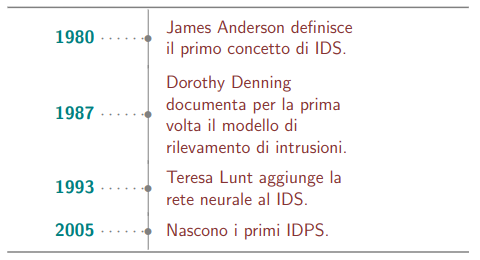
\includegraphics[width=0.45\textwidth]{image/IDStimeline.png}
	\end{wraptable} 
	La prima elaborazione del concetto di sistema di rilevamento delle intrusioni (IDS) risale al 1980 e si deve in particolare a James Anderson, analista presso la National Security Agency. Il sistema di Anderson comprendeva un insieme di strumenti per amministratori di sistema per poter esaminare i registri di audit.\cite{ComputerSecurityThreat}\\
	Nel febbraio del 1987, Dorothy E. Denning, assistita da Peter G. Neumann presso IDS International, pubblicò un documento intitolato "An Intrusion Detection Model", nel quale introdussero miglioramenti al modello di Anderson.\cite{AnIntrusionDetectionModel}
	Il modello di Denning consisteva in un sistema esperto basato su regole per rilevare pattern di intrusioni note e una componente di rilevazione statistica basata su profili di utenti, sistemi host e sistemi di destinazione, diventando noto come Intrusion Detection Expert System.\\
	Nel 1990, Teresa F. Lunt, autrice di "IDES: An Intelligent System for Detecting Intruders", aggiunse l'ultimo componente al modello di Denning: una rete neurale artificiale capace di adattarsi agli eventi e modificarsi.\cite{IDES} \\
	Un sistema di rilevamento delle intrusioni (IDS) è un dispositivo software o un'applicativo che monitora una rete o i dispositivi su cui è installato. Quando rileva un'anomalia, la segnala a un sistema di raccolta di eventi di sicurezza (SIEM), che utilizza tecniche di filtraggio degli allarmi per distinguere falsi positivi da attività dannose.\cite{taxonomy}\\
	Gli IDS, come i firewall, vengono utilizzati per prevenire intrusioni nella rete, ma differiscono dalla risposta a tali intrusioni. I sistemi di rilevamento delle intrusioni possono anche avere scopi specifici se integrati con strumenti personalizzati, come l'utilizzo di un honeypot per attirare e caratterizzare il traffico dannoso.\cite{idsFirewall}\\
	Recentemente, sono stati realizzati prodotti denominati sistemi di rilevamento e prevenzione delle intrusioni (IDPS), i quali possiedono la capacità di rispondere proattivamente alle intrusioni rilevate. Gli IDPS hanno, inoltre, la capacità di fermare un attacco rilevato, registrare gli eventi, avvisare gli amministratori, bloccare la minaccia e generare rapporti. A differenza 
	degli IDS, gli IDPS devono essere posizionati "in linea", monitorando in tempo reale per bloccare intrusioni, inviare allarmi, rifiutare pacchetti dannosi e correggere errori di rete.\cite{idps}\\
	
	
	\subsection{Tipologie di IDS}
	La classificazione dei sistemi di intrusione si basa sulla loro posizione:
	\begin{itemize}
		\item \textbf{NIDS (Network IDS)}: posizionati strategicamente nella rete, monitorano il traffico da e verso tutti i dispositivi, analizzando idealmente sia l'entrata che l'uscita. L'uso di reti neurali artificiali può migliorare i tassi di rilevamento grazie alla capacità di analizzare grandi volumi di dati in modo intelligente e apprendere dagli errori, sviluppando un sistema di avviso precoce.\cite{taxonomy}
		\item \textbf{HIDS (Host IDS)}: operano su singoli host o dispositivi, monitorando solo i pacchetti in entrata e in uscita. Consentono l'analisi del traffico di rete criptato, una volta arrivato all'host.\cite{taxonomy}
	\end{itemize}
	Gli IDS possono essere classificati anche in base all'approccio di rilevamento:
	\begin{itemize}
		\item \textbf{Signature-based}: ricerca pattern specifici, simile all'azione degli antivirus per individuare sequenze di byte o istruzioni malevole conosciute. Risponde velocemente a attacchi noti, ma può non riconoscere nuovi attacchi senza pattern noti.\cite{signature}
		\item \textbf{Anomaly-based}: utilizza l'apprendimento automatico per creare un modello di attività affidabile e confrontare il nuovo comportamento. Riesce a rilevare attacchi sconosciuti, ma potrebbe generare falsi positivi, identificando attività legittime come malevoli.\cite{anomaly}
	\end{itemize}
	
	\subsection{Darktrace: panoramica}
	Darktrace, fondata nel 2013 a Cambridge, Regno Unito, da ex-dipendenti dell'intelligence governativa e matematici dell'Università di Cambridge, è un Intrusion Detection and Prevention System (IDPS) che immagazzina e analizza il traffico di rete per lunghi periodi al fine di identificare correlazioni e modelli comportamentali.\\
	Utilizzando avanzate tecniche di probabilità bayesiana e machine learning, Darktrace crea un profilo comportamentale unico per ciascun utente e dispositivo all'interno dell'ambiente di rete. Inoltre, è in grado di raggruppare gli utenti e i dispositivi in base ai loro comportamenti, consentendo così di rilevare anomalie nel caso in cui un utente o un dispositivo si discosti dal comportamento tipico del suo gruppo.\\
	Operando in tempo reale e analizzando il traffico di rete in modo continuo, Darktrace è in grado di identificare anche gli attacchi "zero-day", che non seguono schemi precedentemente noti. Per garantire l'affidabilità delle segnalazioni, Darktrace utilizza un'intelligente soglia di rilevamento che contestualizza e aggiorna costantemente le segnalazioni in base alle rilevazioni precedenti, riducendo al minimo i falsi positivi e mitigando il rischio di distorsioni dovute al tasso di base.\\
	Darktrace è composto da quattro moduli distinti: Darktrace PREVENT, Darktrace DETECT, Darktrace RESPOND e Darktrace HEAL. Tuttavia, durante il tirocinio, ci concentreremo esclusivamente sui moduli DETECT e RESPOND, in quanto sono gli unici utilizzati durante l'esperienza pratica.\cite{threat1}
	
	\subsection{Darktrace DETECT}
	Darktrace DETECT offre un'interfaccia che segnala le anomalie e fornisce gli strumenti per valutare se sono comportamenti legittimi nell'ambiente lavorativo o malevoli. Le violazioni dei modelli possono essere parte di un incidente dell'AI Analyst o un'allerta autonoma, comunicando agli utenti tramite l'interfaccia Threat Visualizer comportamenti anomali di dispositivi o account.\cite{threat2}\\
	Un modello è composto da tre elementi fondamentali:
	\begin{itemize}
		\item Condizioni del modello: sono componenti che, quando soddisfatte, provocano una violazione del modello. Ogni componente è composto da una metrica con le proprie condizioni filtro, come l'utilizzo di protocolli specifici o pacchetti HTTP con User Agent rari. Questi elementi, insieme, costituiscono la logica del modello.
		\item Modulazione del punteggio: comprende quattro modelli che influenzano il comportamento del modello quando viene attivato. Il modello standard specifica che una continua violazione nel tempo diminuisce il punteggio, ma esistono anche altre modalità: una modulazione che mantiene lo stesso punteggio nel tempo e un'altra che aumenta il punteggio dopo le prime violazioni e poi lo diminuisce.
		\item Azioni del modello: sono azioni di sistema che possono essere attivate in risposta a una violazione del modello. Queste azioni possono includere l'invio di email o notifiche HTTP. Inoltre, è possibile selezionare una criticità diversa da quella standard o segnalare la violazione come "Informational".\cite{model}
	\end{itemize}
	Solo una parte degli incidenti viene segnalata dall'\textit{AI Analyst} di Darktrace, il quale raccoglie molteplici informazioni rilevanti e le presenta in un formato facilmente comprensibile per l'operatore. Questo strumento investiga, analizza e categorizza le minacce all'interno dell'ambiente, identificando incidenti potenzialmente interessanti e insoliti, spesso raggruppandoli per un singolo dispositivo. Gli incidenti che coinvolgono più dispositivi sono classificati come incidenti "\textit{cross-network}".\\
	L'\textit{AI Analyst} non si limita a investigazioni autonome e non sollecitate, ma è anche disponibile su richiesta per un dispositivo selezionato da parte dell'operatore.\\
	Per quanto riguarda le allerte autonome, è compito dell'analista indagare su di esse utilizzando gli strumenti forniti da Darktrace DETECT per rispondere alle 5 W:
	\begin{enumerate}
		\item Who?: identificare chi ha scatenato l'allarme.
		\item What?: comprendere quale azione è stata compiuta.
		\item When?: determinare quando sono avvenute tali operazioni.
		\item Where?: individuare il dispositivo o il luogo in cui sono state effettuate tali operazioni.
		\item Why?: capire il motivo per cui Darktrace ha segnalato questa anomalia.
	\end{enumerate}
	Se la legittimità dell'attività non è immediatamente chiara attraverso le informazioni fornite dalla violazione del modello, è consigliabile contattare l'utente finale, poiché la consultazione e la collaborazione con gli utenti sono fondamentali per una valutazione completa della situazione.\cite{threat2}
	
	\subsection{Darktrace RESPOND}
	Darktrace RESPOND/Network è progettato per gestire minacce di sicurezza di alto livello, come ad esempio i ransomware. Utilizzando due approcci distinti, può interrompere le connessioni malevole sia attraverso il reset TCP che integrandosi direttamente con il firewall esistente, inviando messaggi direttamente a esso.\\
	Il flag RST del protocollo TCP è una componente delle comunicazioni standard tra dispositivi: quando un endpoint riceve un pacchetto con questo flag attivato, la connessione viene immediatamente interrotta. Darktrace rileva attività sospette e, in caso di anomalie, invia pacchetti di reset TCP a entrambi i dispositivi coinvolti, sia all'interno che all'esterno della rete, per interrompere la connessione malevola. Gli indirizzi IP dei pacchetti di reset sono falsificati per far credere ai dispositivi che non provengano da Darktrace, ma l'uno dall'altro.\\
	Darktrace RESPOND può attuare una serie di azioni proattive, misurate e automatizzate in risposta a minacce informatiche confermate rilevate in tempo reale.\\
	I componenti di Darktrace RESPOND possono essere utilizzati in due modalità distinte:
	\begin{itemize}
		\item \textbf{Modalità di conferma umana}: le azioni di Darktrace RESPOND rimarranno in 
		sospeso fino a quando un operatore umano non conferma o ignora 
		la segnalazione del modulo RESPOND.
		\item \textbf{Modalità autonoma o parzialmente autonoma}: in modalità completamente 
		autonoma, RESPOND risponde automaticamente alle minacce, mentre nella modalità 
		parzialmente autonoma, può essere attivato autonomamente al di fuori degli orari 
		lavorativi, ma richiede conferma umana per il resto del tempo.
	\end{itemize}
	
	
	Darktrace RESPOND reagisce alle violazioni dei modelli offrendo l'opzione di impostare 
	un inibitore, che è un'azione finalizzata a contrastare il comportamento anomalo del 
	dispositivo o dell'utente. Gli inibitori disponibili includono:
	\begin{itemize}
		\item \textbf{Bloccare le connessioni corrispondenti}: interrompe le connessioni dal dispositivo all'endpoint di destinazione identificato nell'incidente, sulla porta di destinazione osservata.
		\item \textbf{Imporre il pattern di vita}: consente al dispositivo di effettuare solo connessioni e trasferimenti di dati considerati normali da Darktrace, basati sui modelli di vita definiti per quel dispositivo. Qualsiasi attività che si discosti da questi modelli viene bloccata.
		\item \textbf{Imporre il pattern di vita del gruppo}: permette al dispositivo di intraprendere le stesse connessioni e trasferimenti di dati che sono comuni tra i dispositivi nel suo gruppo di pari, basandosi sui modelli di vita del gruppo.
		\item \textbf{Quarantena del dispositivo}: blocca tutto il traffico di rete in entrata e in uscita dal dispositivo, isolandolo dalla rete.
		\item \textbf{Blocco di tutti i traffici in uscita}.
		\item \textbf{Blocco di tutti i traffici in entrata}.\cite{respond}
	\end{itemize}
	
	\chapter{Sperimentazione con Tpot e Darktrace}
	\section{Implementazione di Tpot e analisi dei risultati}
	\subsection{Configurazione di base}
	Per prima cosa, è fondamentale verificare di avere tutti i prerequisiti necessari per l'installazione corretta dell'honeypot.  Questi prerequisiti includono spazio di archiviazione minimo necessario, spazio di memoria RAM (memoria ad accesso casuale), un indirizzo IP fornito da un server DHCP e una connessione ad Internet. Queste possono variare in base alla tipologia di installazione se \textit{standalone} o \textit{distribuita}.\\
	Successivamente, dalla pagina ufficiale Github di T-Pot deve essere scaricata l'immagine ISO, questo file contiene l'immagine del sistema operativo preconfigurato con tutti gli strumenti e le funzioni necessarie per T-Pot.\\
	Una volta scaricata l'immagine ISO, il passo successivo è l'installazione effettiva dell'immagine. Questo deve avvenire seguendo attentamente i passaggi indicati fino al completamento dell'installazione, potendo decidere durante il processo se installare la versione \textit{standalone}, \textit{alveare} o \textit{sensore}.\\
	Una volta completata l'installazione, viene visualizzata un prompt contenente le informazioni per connettersi al sistema da remoto, potendo utilizzare l'interfaccia web contenente un terminale oppure tramite connessione SSH. Questo conferma che T-Pot è stato installato correttamente ed è pronta all'uso.\\
	\begin{center}
		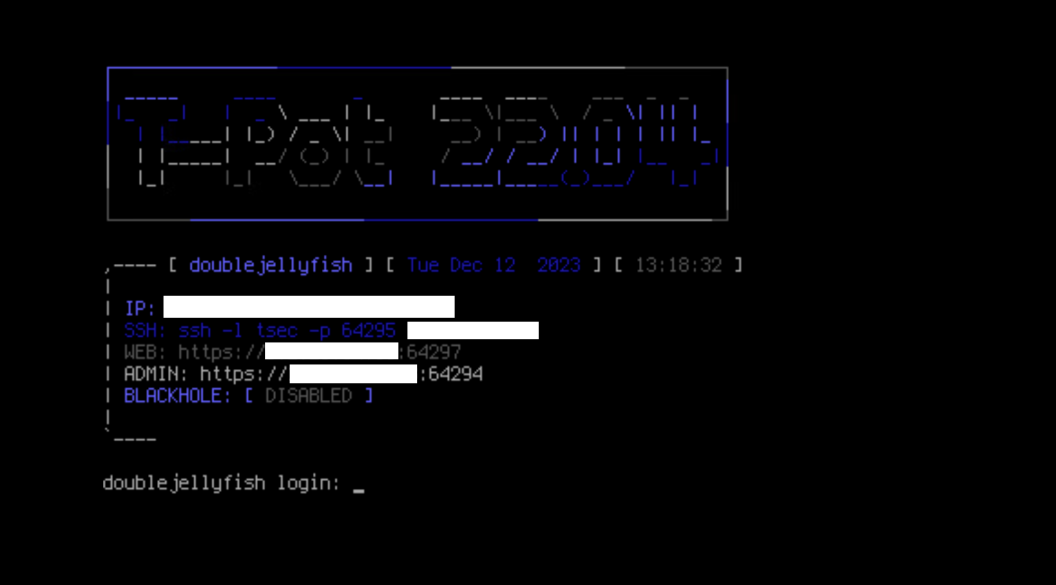
\includegraphics[width=0.65\textwidth]{image/fineInstallazione.png}
	\end{center}
	Dopo aver completato l'installazione di T-Pot, è necessario apportare alcune modifiche e configurazioni aggiuntive per assicurarsi che funzioni correttamente.\\
	Il primo passaggio dopo l'installazione è modificare il file \textit{/etc/network/interface} per configurare correttamente l'interfaccia di rete primaria dell'honeypot. Dopo aver apportato le modifiche al file di configurazione, è necessario riavviare l'interfaccia di rete affinché le modifiche abbiano effetto. Successivamente, è importante installare e configurare il server di posta Postfix utilizzando il gestore di pacchetti apt. Postfix è necessario per consentire a T-Pot di inviare mail contenenti le segnalazioni di connessioni malevole. \\
	Durante la configurazione di Postfix, è essenziale assicurarsi che sia configurato per utilizzare la porta 587 per le comunicazioni email anziché la porta standard 25. Questo è particolarmente importante perché la porta 25 è comunemente monitorata dagli attaccanti, mentre la porta 587 offre una maggiore sicurezza.
	
	\subsection{Script e automazioni}
	L'idea iniziale era di collegare T-Pot con un SIEM tramite plugin o programmi esistenti, ma poiché non erano disponibili soluzioni adatte alle esigenze aziendali, è stato sviluppato uno script per analizzare i log dei principali honeypot: 
	\begin{itemize}
		\item Dionaea: utilizzato per monitorare la porta legata al protocollo FTP(21).
		\item Cowrie: utilizzato per monitorare le porte legate ai protocolli SSH e Telnet(22, 23).
		\item Tanner: utilizzato per monitorare le porte legate al protocollo HTTP(80, 8080).
		\item Citrixhoneypot: utilizzato per monitorare le porte legate al protocollo HTTPS(443).
		\item Honeytrap: utilizzato per monitorare un gruppo di porte non standard, le porte maggiori di 1024.
	\end{itemize}
	Lo script estrae le informazioni rilevanti dai log di ogni honeypot e le formatta per l'integrazione con il SIEM.\\
	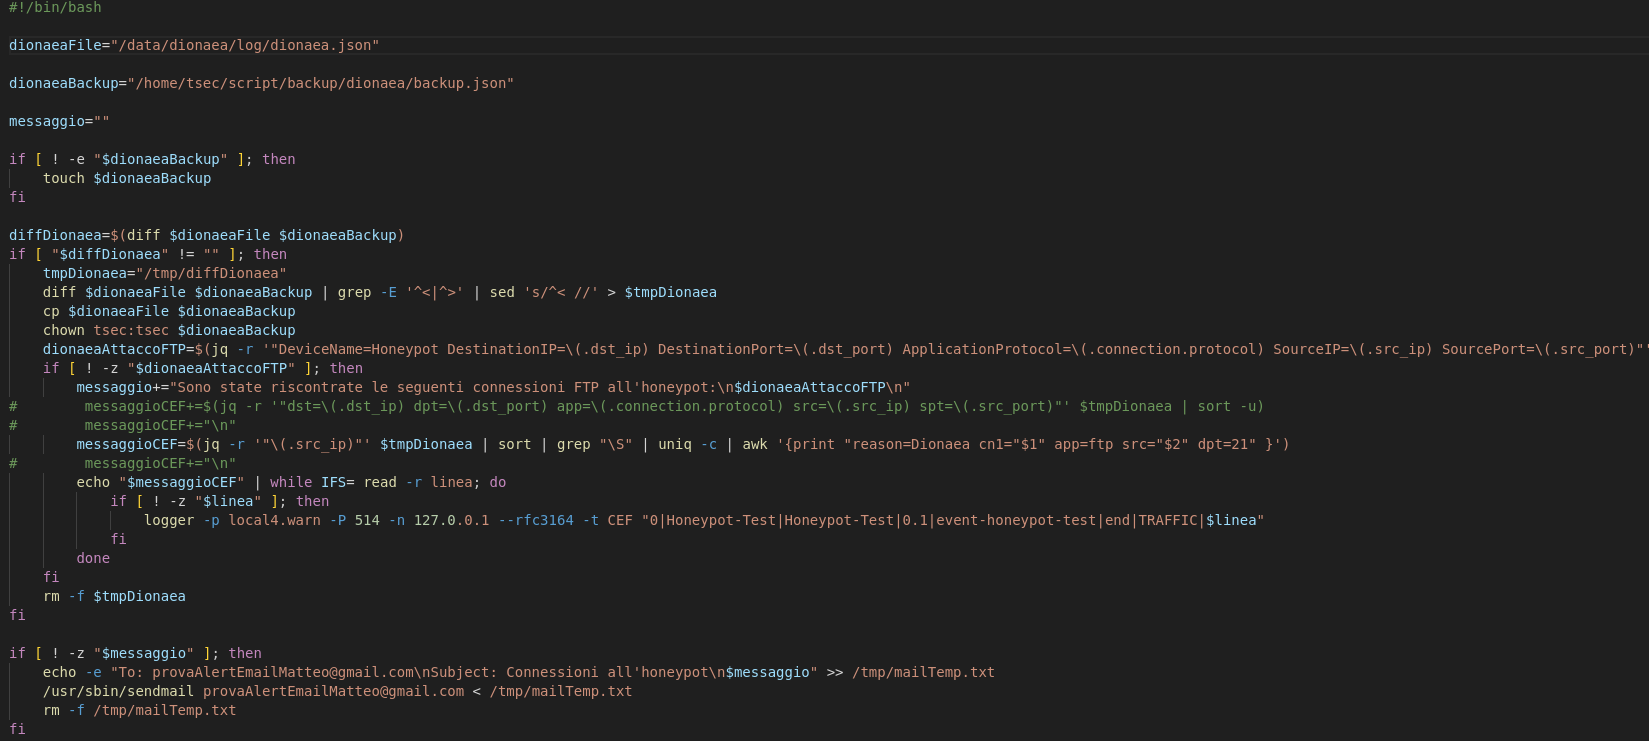
\includegraphics[width=\textwidth]{image/script.png}
	\newpage
	Ecco una spiegazione delle principali azioni svolte dallo script:
	\begin{enumerate}
		\item Viene definito il percorso del file di log dell'honeypot e il percorso del file di backup che conterrà una copia del file di log per confronti successivi.
		\item Se il file di backup non esiste, viene creato.
		\item Viene eseguito un confronto tra il file di log attuale e quello di backup per individuare eventuali differenze.
		\item Se vengono rilevate delle differenze, vengono estratte le informazioni sulle connessioni di attacco dal file di log attuale.
		\item Queste informazioni vengono aggiunte a un messaggio di notifica che sarà inviato tramite email.
		\item Viene generato un messaggio nel formato CEF (Common Event Format) per ciascuna connessione di attacco trovata.
		\item Infine, se è stato creato un messaggio di notifica, viene creato un file temporaneo contenente il testo dell'email di notifica e viene inviata l'email utilizzando il comando sendmail.
	\end{enumerate}
	Questo processo viene effettuato per i cinque honeypot elencati precedentemente.
	
	\subsection{Dati raccolti}
	Il compito dello script mostrato precedentemente segnala solo in caso di attacco verso le porte più utilizzate ma non la totalità.
	I dati che verranno mostrati successivamente sono stati raccolti in un periodo temporale di una settimana, durante il quale T-Pot è stato esposto a Internet e ha registrato tutti gli attacchi subiti.\\
	
	L'analisi dei dati raccolti ha rivelato che la quasi totalità dei pacchetti ricevuti è di tipo TCP, rappresentando il 91,3\% del totale, seguito da UDP con il 4,2\% e ICMP con il 3,5\%. Questo è in linea con il fatto che il protocollo TCP richiede un maggior numero di pacchetti per la sua affidabilità.\\
	
	Dal punto di vista geografico, gli Stati Uniti d'America, la Russia e la Repubblica Popolare Cinese sono i principali attori, contribuendo complessivamente al 59,8\% di tutti gli attacchi registrati, seguiti da altri paesi come Regno Uniti, Paesi Bassi, Vietnam, India, Singapore, Germania e il resto del mondo, che rappresenta il 6,8\%.\\
	
	Nel dettaglio delle porte più attaccate, la porta 22 (SSH) risulta essere la più frequentemente bersagliata, rappresentando il 44,8\% di tutti gli attacchi registrati. Le porte 443 (HTTPS) e 80 (HTTP) seguono rispettivamente con il 14,8\% e il 10,3\%. Altre porte di rilevanza includono la porta 23 (Telnet) e la porta 25 (SMTP), mentre le porte non standard, quelle oltre numerate oltre la 1024, contribuisce in misura minore agli attacchi subiti.
	
	\subsection{Esperienze pratiche durante il tirocinio}
	Durante il tirocinio, ho avuto modo di affrontare diverse sfide nell'implementazione e nella gestione di un honeypot. Oltre alla configurazione iniziale, una delle principali sfide è stata l'integrazione con il SIEM (Security Information and Event Management) e con gli altri sistemi di sicurezza presenti nell'ambiente di produzione. Inoltre, ho avuto l'opportunità di collaborare con altri membri del team di sicurezza per analizzare i dati raccolti e identificare potenziali vettori d'attacco su sistemi aziendali già presenti.
	
	\section{Monitoraggio delle reti con Darktrace}
	\subsection{Studi di caso}
	
	
	\subsection{Esempi di minacce rilevate}
	
	\section{Integrare Darktrace e Tpot per una maggiore sicurezza}
	
	\chapter{Conclusioni}
	\section{Riassunto delle principali conclusioni}
	\section{Riflessioni personali sull'esperienza di tirocinio}
	
	\chapter{Bibliografia}
	\printbibliography[heading=none]
	
	\chapter{Ringraziamenti}
	
\end{document}
